\chapter{Eksperyment}

W końcowym etapie pracy postanowiono przeprowadzi\'c analizę jakościową zaimplementowanego
systemu. W tym celu posłużono się i obliczono wartości dwóch najpopularniejszych współczynników
używanych do oceny poprawności działania systemów biometrycznych:

\begin{itemize}
  \item FAR \textit{(ang. False Acceptance Rate)} - miara prawdopodobieństwa nieprawidłowego zaakceptowania
  obrazu
  \item FRR \textit{(ang. False Rejection Rate)} - miara prawdopodobieństwa nieprawidłowego odrzucenia
  obrazu
\end{itemize}

W dalszej części tego rozdziału zawarty został opis eksperymentu oraz zasobów użytych do jego
przeprowadzenia.

\section{Wykorzystane wska\'zniki}

Tak jak wspomniano we wstępie niniejszego rozdziału, do określenia dokładności działania zaimplementowanego
systemu użyte zostały wska\'zniki FAR oraz FRR. \newline

FAR \textit{(ang. False Acceptance Rate)} definiuje prawdopodobieństwo zaistnienia sytuacji, w której
osoba nieautoryzowana może zosta\'c nieprawidłowo rozpoznana przez system biometryczny. Zwykle wska\'znik ten
jest uważany za najważniejszy, ze względu na bezpośrednie opisywanie prawdopodobieństwa narusznia
bezpieczeństwa systemu. Wska\'znik ten można zdefiniowa\'c w następujący sposób:

\begin{equation}
  \mathit{FAR} = \frac{N_{\mathit{fa}}}{N_{t}},
\end{equation}

\noindent
gdzie:\\
\indent $\mathit{FAR}$ - False Acceptance Rate,\\
\indent $N_{\mathit{fa}}$ - liczba nieprawidłowo zaakceptowanych dopasowań,\\
\indent $N_{t}$ - liczba wszystkich prób dopasowań.\newline

Drugim wska\'znikiem wykorzystywanym do określenia jakości działania systemu jest FRR \textit{(ang. False Rejection Rate)}.
Mówi on o prawdopodobieństwu nieprawidłowego odrzucenia osoby identyfikowanej. Jest to wska\'znik, który
nie wskazuje wad w bezpieczeństwie działania systemu, natomiast może definiowa\'c to jak
szybko będzie dany system działał oraz ilukrotnie potencjalny użytkownik będzie musiał powtórzy\'c
proces autoryzacji. Wska\'znik ten można zdefiniowa\'c w sposób opisany przez poniższe równianie:

\begin{equation}
  \mathit{FRR} = \frac{N_{\mathit{fr}}}{N_{t}},
\end{equation}

\noindent
gdzie:\\
\indent $\mathit{FRR}$ - False Rejection Rate,\\
\indent $N_{\mathit{fr}}$ - liczba nieprawidłowo odrzuconych dopasowań,\\
\indent $N_{t}$ - liczba wszystkich prób dopasowań.\newline

Za najlepsze rozwiązanie systemu biometrycznego można uzna\'c takie, które jednocześnie zapewnia
najmniejszą wartoś\'c obu tych współczynników (z naciskiem na FAR). Takie podejście pozwala zachowa\'c balans między bezpieczeństwem
systemu, a jego użyteczńością. Dodatkowo wyznacza się współczynnik EER \textit{(ang. Equal Error Rate)}, który jest równy
FAR lub FRR w momencie, gdy oba te wska\'zniki są sobie równe. Pozwala on na jednoznaczne porównanie systemów
biometrycznych pod względem jakości działania.

\begin{figure}[ht]
  \centering
  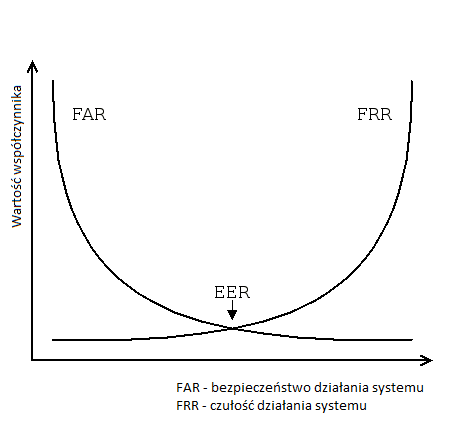
\includegraphics[width=0.7\textwidth]{images/experiment/FARFRRERR.png}
  \caption{Balans między współczynnikami FAR oraz FRR.}
\end{figure}

\section{Opis eksperymentu}

W celu określenia jakości działania zaimplementowanego systemu postanowiono obliczy\'c wartości powyżej opisanych wska\'zników
przy użyciu różnych wartości parametrów metod poszczególnych etapów przetwarzania. We wszystkich przypadkach zdecydowano
się na użycie metody segmentacji zaproponowanej przez Daugmana \cite{DaugmanHowIrisRecognitionWorks}, która na podstawie obserwacji
określona została jako najlepiej działająca z tych dostępnych w aplikacji. Zastosowana została ona w dwóch wariantach:
bez wykrywania powiek oraz wykrywaniem powiem przy użyciu aproksymacji parabolą. Jako podstawowe wartości parametrów
metod wykorzystano te zaproponowane w swojej pracy przez Maseka \cite{masek}, który opisał je jako optymalne. Pozostałe
przypadki w eksperymencie pokazują odchylenia od tych wartości. Poniżej przedstawiono zestawienie parametrów podstawowych:

\begin{itemize}
  \item normalizacja - rozdzielczoś\'c kątowa równa 240, rozdzielczoś\'c promieniowa równa 32 (odpowiednio szerokoś\'c i wysokoś\'c obrazu)
  \item kodowanie - częstotliwoś\'c środkowa filtru równa 18 pikseli, przepustowoś\'c $\mathit{\sigma/f}$ wynosząca 0.5,
  \item dopasowanie - próg odległości Hamminga równy 0.35, liczba przesunię\'c wynosząca 8.
\end{itemize}

Do przeprowadzenia eksperymentu wykorzystana została baza danych zdję\'c oczu CASIA w wersji pierwszej [zasób: \ref{web:CASIA}].
Składa się ona z 756 obrazów przedstawiających 108 unikalnych tęczówek. Zdjęcia robione były obu oczom w dwóch
sesjach. W ramach sesji pierwszej pobieranie były trzy, a w ramach drugiej sesji cztery zdjęcia. Wszystkie z nich
są w formacie \textit{BMP} i mają rozdzielczoś\'c 320x280 pikseli. Na rysunku poniżej (rysunek \ref{fig:casiaExample})
przedstawione zostały przykładowe obrazy z tej bazy:\newline

\begin{figure}[h]
  \centering
  \begin{subfigure}[b]{\textwidth}
    \centering
    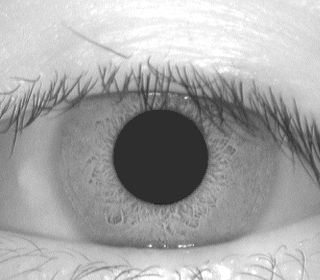
\includegraphics[width=0.45\textwidth]{images/experiment/CasiaExampleOneLeft.png}
    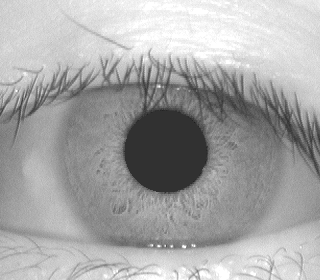
\includegraphics[width=0.45\textwidth]{images/experiment/CasiaExampleOneRight.png}
  \end{subfigure}
  \begin{subfigure}[b]{\textwidth}
    \centering
    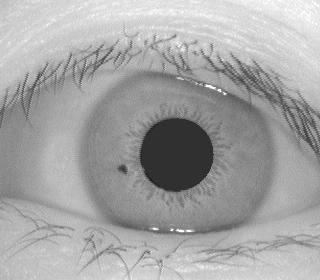
\includegraphics[width=0.45\textwidth]{images/experiment/CasiaExampleTwoLeft.png}
    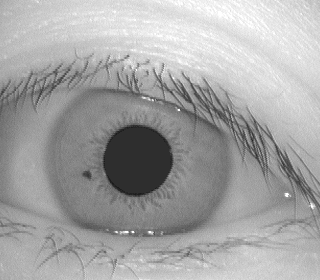
\includegraphics[width=0.45\textwidth]{images/experiment/CasiaExampleTwoRight.png}
  \end{subfigure}
  \caption{Przykładowe zdjęcia z bazy danych CASIA. Z lewej strony
  znajduje się obraz pobrany w pierwszej sejsi, a zdrugiej strony obraz pobrany w drugiej sesji.}
  \label{fig:casiaExample}
\end{figure}

Ze względu na problemy występujące podczas procesu segmentacji, eksperyment przeprowadzony został dla pierwszych
300 obrazów znajdujących się w bazie danych odpowiadających 47 unikalnym tęczówkom. W trakcie eksperymentu
pojawiły się także inne problemy związane z wyznaczaniem powiek, które skutkowały wyznaczeniem maski zakłóceń
obejmującej cały obszar zdjęcia. W takich wypadkach obrazy nie były poddawane eksperymentowi, a liczba pominiętych
obrazów uwzględniona została w trakcie obliczania współczynników FAR oraz FRR.

\section{Wyniki eksperymentu}

Tak jak wcześniej wspomniano, w ramach eksperymentu wykorzystano 300 obrazów, które poddano procesowi
w kilku różnych konfiguracjach. W procesie rozpoznawania porównano każdy obraz z każdym innym, co dało
łącznie 90000 prób identyfikacji.

W przypadku wykorzystania metody Daugmana wraz z aproksymacją powiek za pomocą paraboli zaobserwowane
zostały problemy w działaniu algorytmu znajdowania powiek, które skutkowały niepoprawnym generowaniem maski.
Tych przypadków nie uwzględniano w obliczeniach, w związku z czym łączna liczba prób identyfikacji dla tej
konfiguracji zmalała do wartości 87023.\newline

\noindent
Poniżej przedstawione zostały wartości obliczonych współczynników dla domyślnych parametrów
procesu opisanych w poprzedniej części rozdziału:

\rowcolors{2}{gray!10}{white}
\begin{table}[ht]
  \centering
  \begin{tabular}{c|c|c|c}
    \rowcolor{gray!20}
    Metoda segmentacji & Metoda wykrywania powiek & FAR & FRR \\
    \hline\hline
    Daugman & Brak & 0.0000 & 0.0094 \\
    \hline
    Daugman & Aproksymacja parabolą & 0.0001 & 0.0076 \\
  \end{tabular}
  \caption{Porównanie współczynników FAR i FRR dla różnych metod wykrywania powiek.}
\end{table}

Uzyskane wyniki współczynnika FAR są bardzo bliskie zera z dokładnością do czwartego miejsca
po przecinku. Wynik ten jest wysoce zadawalający, ponieważ sugeruje to wysoką odpornoś\'c systemu
na błędną identyfikację użtkownika. Obliczony współczynnik FRR jest wyższy niż FAR i oscyluje
około wartości 0.008. Biorąc pod uwagę mniejsze znaczenie tego współczynnika dla bezpieczeństwa
systemu również jest to zadawalający wynik.\newline

\noindent
W ramach eksperymentu sprawdzono również wartości wska\'zników FAR oraz FRR przy zmianie:

\begin{itemize}
  \item wartości progu odległości Hamminga w procesie dopasowania,
  \item liczby przesunię\'c wykonywanych w procesie dopasowania,
  \item wartości rozdzielczości kątowej i promieniowej w procesie normalizacji,
  \item wartości parametru $\mathit{\sigma/f}$ filtru Gabora w procesie kodowania.
\end{itemize}

\noindent
Poniżej przedstawione zostały zestawienia obliczonych metryk przy zmianie progu decyzyjnego
w procesie dopasowania:

\begin{itemize}
  \item bez wykrywania powiek

  \rowcolors{2}{gray!10}{white}
  \begin{table}[ht]
    \centering
    \begin{tabular}{c|c|c}
      \rowcolor{gray!20}
      Próg odległości Hamminga & FAR & FRR \\
      \hline\hline
      0.25 & 0.0000 & 0.0198 \\
      \hline
      0.35 & 0.0000 & 0.0094 \\
      \hline
      0.45 & 0.0282 & 0.0004 \\
      \hline
      0.5 & 0.9698 & 0.0000 \\
    \end{tabular}
    \caption{Porównanie współczynników FAR i FRR dla różnych wartości progowych odległości Hamminga
    przy braku wykrywania powiek.}
  \end{table}

  \item z wykrywaniem powiek z użyciem aproksymacji za pomocą paraboli

  \rowcolors{2}{gray!10}{white}
  \begin{table}[ht]
    \centering
    \begin{tabular}{c|c|c}
      \rowcolor{gray!20}
      Próg odległości Hamminga & FAR & FRR \\
      \hline\hline
      0.25 & 0.0000 & 0.0196 \\
      \hline
      0.35 & 0.0002 & 0.0077 \\
      \hline
      0.45 & 0.0387 & 0.0003 \\
      \hline
      0.5 & 0.9702 & 0.0000 \\
    \end{tabular}
    \caption{Porównanie współczynników FAR i FRR dla różnych wartości progowych odległości Hamminga
    z wykorzystaniem aproksymacji parabolicznej do wykrywania powiek.}
  \end{table}
\end{itemize}

Jak wida\'c przypadek w którym nie jest generowana maska dla powiek daje nieznacznie lepsze wyniki
współczynnika FAR niż konfiguracja uwzględniająca je w masce. Może by\'c to spowodowane niespójnościami
w procesie wyznaczania paraboli odcinających tęczówkę między obrazami tej samej tęczówki. Odwrotną sytuację
obserwujemy w przypadku współczynnika FRR - lepsze wyniki uzyskujemy przy uwzględnieniu powiek w procesie.
Warto zauważy\'c prawie niezauważalną zmianę współczynnika FAR przy zmniejszeniu wartości progu do wartości 0.25.
W wyniku tej zmiany parametru zauważamy natomiast wzrost współczynnika FRR. Ze względu na dążenie do balansu
między wartościami tych współczynników, lepszym wyborem jest wartoś\'c 0.35.

Zwiększając wartoś\'c progu decyzyjnego zauważamy drastyczny wzrost współczynnika FAR. Związane jest to ze zbliżaniem
się do wartości 0.5 progu, dla której obserwujemy praktycznie stuprocentową szansę na nieprawidłowe rozpoznanie.
Związane jest to z definicją odległości Hamminga oraz reprezentacją tęczówki za pomocą ciągu bitów. W ciągu bitowym
istnieje 50\% szans, że na danym miejscu wystąpi wartoś\'c 1 lub 0. Ponieważ dla dwóch niezależnych tęczówek
ich reprezentacja powinna by\'c kompletnie losowa, odległoś\'c Hamminga między nimi będzie wynosi\'c właśnie 0.5.
Jeżeli między dwoma wzorami występuje natomiast pewna korelacja, wówczas wartoś\'c ta spada.\newline

\noindent
Poniżej przedstawione zostały zestawienia obliczonych metryk przy zmianie liczby przesunię\'c bitowych
wzoru tęczówki w procesie dopasowania:

\begin{itemize}

  \item bez wykrywania powiek:

  \rowcolors{2}{gray!10}{white}
  \begin{table}[ht]
    \centering
    \begin{tabular}{c|c|c}
      \rowcolor{gray!20}
      Liczba przesunię\'c & FAR & FRR \\
      \hline\hline
      1 & 0.0000 & 0.0111 \\
      \hline
      3 & 0.0000 & 0.0098 \\
      \hline
      8 & 0.0000 & 0.0094 \\
    \end{tabular}
    \caption{Porównanie współczynników FAR i FRR dla różej liczby przesunię\'c wzoru tęczówki w procesie dopasowania
    przy braku wykrywania powiek.}
  \end{table}

  \item z wykrywaniem powiek z użyciem aproksymacji za pomocą paraboli

  \rowcolors{2}{gray!10}{white}
  \begin{table}[ht]
    \centering
    \begin{tabular}{c|c|c}
      \rowcolor{gray!20}
      Liczba przesunię\'c & FAR & FRR \\
      \hline\hline
      1 & 0.0000 & 0.0096 \\
      \hline
      3 & 0.0001 & 0.0082 \\
      \hline
      8 & 0.0002 & 0.0077 \\
    \end{tabular}
    \caption{Porównanie współczynników FAR i FRR dla różej liczby przesunię\'c wzoru tęczówki w procesie dopasowania
    z wykorzystaniem aproksymacji parabolicznej do wykrywania powiek.}
  \end{table}
\end{itemize}

Jak wida\'c na powyższych zestawieniach zmiana liczby przesunię\'c w nieznacznym stopniu wpływa
na wska\'znik FAR, natomiast zwiększanie liczby wykonywanych przesunię\'c bitowych zmniejsza wartoś\'c
wspólczynnika FRR. Duże znaczenie dla optymalnej liczby przesunię\'c ma jakoś\'c wykonanych zdję\'c tęczówki
oraz potencjalna rotacja oka w trakcie pobierania zdjęcia.

\noindent
Poniżej przedstawiono zestawienie metryk przy zmianach rozmiaru obrazu znormalizowanego:

\begin{itemize}
 \item brak wykrywania powiek:

  \rowcolors{2}{gray!10}{white}
  \begin{table}[ht]
    \centering
    \begin{tabular}{c|c|c|c}
      \rowcolor{gray!20}
      Rozdzielczoś\'c kątowa & Rozdzielczoś\'c promieniowa & FAR & FRR \\
      \hline\hline
      120 & 16 & 0.0027 & 0.0073 \\
      \hline
      240 & 32 & 0.0000 & 0.0094 \\
      \hline
      360 & 64 & 0.0000 & 0.0109 \\
    \end{tabular}
    \caption{Porównanie współczynników FAR i FRR dla różnych rozmiarów obrazu znormalizowanego
    przy braku wykrywania powiek.}
  \end{table}

  \item z wykrywaniem powiek z użyciem aproksymacji za pomocą paraboli

  \rowcolors{2}{gray!10}{white}
  \begin{table}[ht]
    \centering
    \begin{tabular}{c|c|c|c}
      \rowcolor{gray!20}
      Rozdzielczoś\'c kątowa & Rozdzielczoś\'c promieniowa & FAR & FRR \\
      \hline\hline
      120 & 16 & 0.0035 & 0.0065 \\
      \hline
      240 & 32 & 0.0002 & 0.0077 \\
      \hline
      360 & 64 & 0.0001 & 0.0091 \\
    \end{tabular}
    \caption{Porównanie współczynników FAR i FRR dla różnych rozmiarów obrazu znormalizowanego
    z wykorzystaniem aproksymacji parabolicznej do wykrywania powiek.}
  \end{table}
\end{itemize}

Jak wida\'c najlepszy balans między dwoma współczynnikami przy zmianie rozmiaru obrazu znormalizowanego
można zauważy\'c dla rozmiaru pośredniego. Wyższa wartoś\'c współczynnika FAR dla mniejszej rozdzielczości
kątowej może wynika\'c z niewystarczającej ilości informacji zapisanych w znormalizowanym obrazie. Zwiększenie
rozdzielczości powoduje natomiast wzrost współczynnika FRR, co może by\'c spowodowane nadreprezentacją pewnych
cech we wzorze tęczówki.\newline

\noindent
Poniżej przedstawiono zestawienie metryk przy zmianach parametru $\sigma/f$ filtru Gabora używanego
w procesie kodowania:

\begin{itemize}

  \item brak wykrywania powiek:

  \rowcolors{2}{gray!10}{white}
  \begin{table}[ht]
    \centering
    \begin{tabular}{c|c|c}
      \rowcolor{gray!20}
      $\mathit{\sigma/f}$ & FAR & FRR \\
      \hline\hline
      0.3 & 0.0003 & 0.0080 \\
      \hline
      0.5 & 0.0000 & 0.0094 \\
      \hline
      0.75 & 0.0000 & 0.0100 \\
    \end{tabular}
    \caption{Porównanie współczynników FAR i FRR dla różnych wartości parametru $\mathit{\sigma/f}$ filtru Gabora
    przy braku wykrywania powiek.}
  \end{table}

  \item z wykrywaniem powiek z użyciem aproksymacji za pomocą paraboli

  \rowcolors{2}{gray!10}{white}
  \begin{table}[ht]
    \centering
    \begin{tabular}{c|c|c}
      \rowcolor{gray!20}
      $\mathit{\sigma/f}$ & FAR & FRR \\
      \hline\hline
      0.3 & 0.0009 & 0.0069 \\
      \hline
      0.5 & 0.0002 & 0.0077 \\
      \hline
      0.75 & 0.0008 & 0.0084 \\
    \end{tabular}
    \caption{Porównanie współczynników FAR i FRR dla różnych wartości parametru $\mathit{\sigma/f}$ filtru Gabora
    z wykorzystaniem aproksymacji parabolicznej do wykrywania powiek.}
  \end{table}
\end{itemize}

Niestety z powyższych pomiarów nie można wyciągną\'c jednoznaczych wniosków na temat wpływu tego
paramteru na wartoś\'c współczynników FAR oraz FRR.
